\chapter{Test}\label{ch:03_fun_with}

\section{Introduction}



\section{Pricing under Partial Network Information}\label{sec:part_info}
\subsection{Random Networks}
Next, we would like to move to the study of random networks. To motivate this change, note that one issue with studying the profits and regrets of deterministic graphs is that they are sensitive to local changes in the network. The addition or deletion of a single edge, even in a large network, could reduce the regret from a large quantity to 0. An example is given in Figure~\ref{fig:non-robust}. In this figure, the network on the left has a high regret using uniform pricing, but the addition of one edge reduces this regret to zero. This is because the centralities of the network go from being uneven to all identical. 
\begin{figure}[t!]
    \centering
    \hfill
    \subfloat[An example of a network where there is significant regret from using uniform pricing.\ \label{fig:non-robusta}]{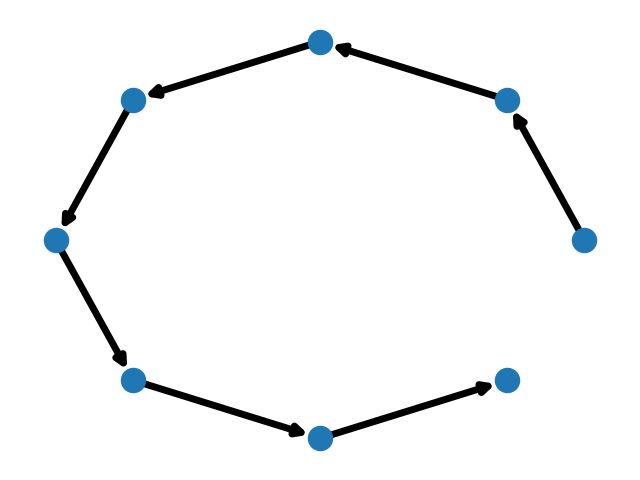
\includegraphics[height=1.1in]{Figures/Pricing/p1.png}
    }
    \hfill 
    \subfloat[A second graph where the addition of one extra edge reduces the regret to 0.\label{fig:non-robustb}]{
        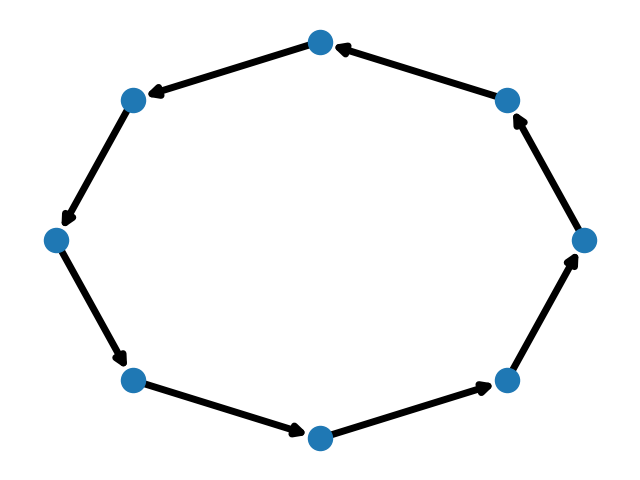
\includegraphics[height=1.1in]{Figures/Pricing/p2.png}
    }
    \hfill 
\end{figure}\label{fig:non-robust}


To further study the phenomenon of pricing on networks in a more robust way, we study the problem over a sequence of random graphs increasing in size. We will study the expected regret for a sequence of random graphs under different pricing schemes. We are especially interested in the asymptotic behavior of this expected regret as the size of the network grows.
\begin{definition}
    A random graph sequence $\{G_n\}$ is a set of graphs indexed by the number of nodes where each graph $G_n$ is a sample from some distribution. 
\end{definition}


The results of this work are focused on what the merchant should do when it has uncertainty about the network, in particular, uncertainty about which edges exist. The merchant might have some partial or inaccurate view of the network instead of seeing the true network. Formally, the merchant has some information that generates a probability distribution $\mathcal{F}$ of networks. 

The merchant's problem in this regime is to maximize the expected profit given its information, where the expectation is over the possible graphs it might encounter. 
\begin{align}
        \max_{\tb{p}}  \frac{1}{2}  {\left(\tb{p} - c \one \right)}^T \ex{\tb{x}(\tb{p})}
\end{align}


This expected profit depends on the expected consumption of consumers in the network given a price. The consumption vector is a random variable that takes the form \[\tb{x}(\tb{p}) = B_\mathcal{F} (a\one -\tb{p}), \mbox{ where } B_\mathcal{F} \defeq {\left(I - \gamma G \right)}^{-1} \mbox{ and } \gamma \defeq \frac{2\rho}{\|G + G^T\|}.\] The term $(a\one -\tb{p})$ is not random, so only $B_\mathcal{F}$ is random and requires further analysis. This represents the weighted sum of walks for a specific random instance of the network. This means that we can write the problem of pricing under uncertainty as follows.

\begin{definition}
    The merchant's problem under partial information is \[\max_{\tb{p}}  \frac{1}{2}  {\left(\tb{p} - c \one \right)}^T
    \bgen (a\one -\tb{p})\]
\end{definition}

In practice, analyzing the distribution of $B_\mathcal{F}$ could be very complex, but quantifying the expected value of the weighted sum of walks might be more tractable under different distributions over the network. If we are able to compute this expected matrix, then we can compute the optimal price vector. $\bgen$ represents the expected weighted sum of walks in the network over the distribution $\mathcal{F}$.  We provide the expression for the optimal price vector as a function of $\bgen$ in the following Proposition.


\begin{proposition}\label{prop-info-price}
% %% Change information M -> I in this section
    Given a distribution $\mathcal{F}$ of networks, the price to charge that maximizes the expected profit is
    \begin{align*}
        \tb{p}^* = \frac{a+c}{2} \one + \frac{a-c}{2} {(\bgen + \bgen^T)}^{-1} (\bgen - \bgen^T) \one
  \end{align*}
 \end{proposition}

 This expression for the price is made up of a flat rate for everyone, a markup, and a discount term relative to how influential each consumer is in the expected matrix. Furthermore, the profit obtained using this price is given in the following proposition.

\begin{proposition}\label{prop:partial_info}\label{prop-info-prof}
     The expected profit of the merchant is given by 
     \begin{align*}
         \frac{{(a-c)}^2}{8} {\left(\one + \tb{v} \right)}^T \bgen \left(\one - \tb{v} \right),
     \end{align*}

     where $\tb{v} = {(\bgen + \bgen^T)}^{-1} (\bgen - \bgen^T) \one$.
 \end{proposition}

Here, we also highlight the difference between the profit obtained in expectation and the profit obtained in any random sample. The profit for any particular sample of $G$ is given by
 \begin{equation*}
     \frac{{(a-c)}^2}{8} {\left(\one + \tb{v} \right)}^T B_\mathcal{F} \left(\one - \tb{v} \right)
 \end{equation*}
 where $\tb{v} = {(\bgen + \bgen^T)}^{-1} (\bgen - \bgen^T) \one$. Thus, the difference between the expected profit and the profit for a given instance of the network under optimal pricing comes from the middle factor. The expected discounted sum of walks matrix $\bgen$ is replaced by the discounted sum of walks $B_\mathcal{F}$ for the given instance, but the price remains the same and is based on the expected sum of walks.

% %% Proof 

The proof follows from expanding the profit function in terms of the profit the merchant would experience if a particular network were selected and then calculating the expected value over these possible profits. Details can be found in Appendix~\ref{proof:partial_info}.



\subsection{Expected Regret}

The comparative performance of pricing strategies for random networks can be evaluated using expected regret. Writing $\Pi(\tb{p})$ for the expected profit of price vector $\tb{p}$, we define the regret of $\tb{p}$ compared to $\tb{q}$ as $\mathrm{Reg}(\tb{p}, \tb{q}) \defeq \Pi(\tb{q}) - \Pi(\tb{p})$. Likewise, we define the fractional regret as $\mathrm{Reg}_F(\tb{p}, \tb{q}) \defeq 1 - \frac{\Pi(\tb{p})}{\Pi(\tb{q})}$. When $\tb{q}$ is omitted, the comparison is to the optimal price $\tb{p}^*$.

\subsection{Pricing under no network information}

% \am{Here state that when there is no network information then one can  assume that all topologies are equally likely and the expected graph as well as $E[B_F]$ is symmetric. Therefore the uniform price is optimal.}

At one extreme of the information spectrum is the case where the merchant lacks any information about the network whatsoever. When the merchant lacks any information about the network, we assume all network topologies are equally likely. This means that $\bgen$ is symmetric. From~\cite{huang2022value}, this meets the condition for the optimal price vector to be uniform, or, equivalently, for all consumers to be charged the same price. A sufficient condition for the optimal price to be uniform is that for all integers $\ell > 0$, ${({G^T})}^{\ell} \one = G^\ell \one$~\cite{huang2022value}. That is, for all nodes, the number of incoming walks of length $\ell$ is equal to the number of outgoing walks of length $\ell$. Therefore, $\bgen$ being symmetric is sufficient to establish that the optimal price is one uniform price. We state this formally in the following Proposition.
% Given such, we can charge everyone just one price, which we will call the uniform price. This price has a simple form: 

% \am{Shouldn't this be optimal expected profit?}
\begin{proposition}[Uniform Price,~\cite{candogan2012optimal} Corollary 1]
        When all consumers are charged the same price, the optimal price is:
    \begin{equation}
        \tb{p}_0 = \frac{a+c}{2} \one 
    \end{equation}
        This yields an optimal expected profit of
        \begin{equation}
        \Pi(\tb{p}_0) = \frac{{(a-c)}^2}{8} \one^T \bgen \one
    \end{equation}
\end{proposition}


Since this price is optimal, it has zero expected regret. Note that in this Proposition, the price computation does not require that the merchant know anything about the network, but the profit does still depend on the network even when the merchant does not observe it. This profit form, like the optimal profit, is also a weighted sum of walks in the network, with walks of length $\ell$ weighted by $\gamma^\ell$.

We note that it may seem odd that under no network information the expected regret is zero under uniform pricing. This is because the benchmark optimal pricing is itself uniform. With partial information, this would change because additional structure in the network needs to be accounted for while computing optimal prices. That is, there is regret for not having the full network information. 


Here, we provide insight into when, more generally, information matters. Suppose we have a family of random networks, $\{G_n\}$, and for each network we have a price, perhaps based on some partial information about the network. Under what conditions will our pricing be sufficient to achieve negligible regret? We answer this below.
\begin{theorem}
    A sequence has negligible fractional regret if and only if \[ \frac{ \ex{ \| \tb{p} - \tb{p}^* \|_{B+B^T} }  }{ \ex{\Pi(\tb{p}^*)}} \to 0 \]
\end{theorem}

This theorem says precisely that the condition for the regret to be small is that the difference in prices grows asymptotically slower than the profit. If we apply this result to uniform pricing, we can also answer the question of when any information is necessary.

\begin{corollary}
    A sequence of networks has negligible fractional regret using uniform pricing if and only if \[ \frac{\ex{ \tb{v}^T (B+B^T)^{-1} \tb{v}} }{\ex{ \one^T B \one } } \to 0 \] 
\end{corollary}

If this condition is met, then there is no value of information on the network. When no information is known about the network, it is best to charge one uniform price. When given access to the full network, it is best to charge $n$ prices. These are two extremes. What motivates this work is the question `What should the merchant do given partially specified information?'. In particular, we will study charging an intermediate number of prices. We will analyze the trade-offs of charging finer vs coarser prices as well as methods to determine these prices.

\subsection{Partitions}\label{sec:partitions}

    A \emph{partition} $P$ of the consumers $[n]$ into $k$ blocks assigns each consumer to exactly one block, with blocks labeled $1, \dots, k$. For a consumer $i$, $\commidx{P}{i} \in [k]$ is the label of the block containing $i$, and for a label $j$, $\comblock{P}{j} \defeq \{ i : \commidx{P}{i} = j \}$ is the set of consumers in that block. We write $\mathcal{P}_{n,k}$ for the set of all partitions of $[n]$ into $k$ blocks.

    We represent $P$ by its \emph{partition matrix} $R \in \{0,1\}^{k \times n}$, where $R_{ji} = 1$ if $\commidx{P}{i} = j$ and $R_{ji} = 0$ otherwise. Each column of $R$ has exactly one nonzero entry, so $R^T \one_k = \one_n$, and a vector of block prices $\theta \in \mathbb{R}^k$ induces the consumer price vector $R^T \theta$. Since $P$ and $R$ carry the same information, we use $R$ for both from here on.

    Partitions are ordered by refinement. We say $R'$ is \emph{coarser} than $R$, written $R' < R$, if every block of $R'$ is a union of blocks of $R$; that is, $R'$ can be formed by merging blocks of $R$. This is a partial order, so not every pair of partitions is comparable. We say $R$ \emph{covers} $R'$, written $R' \leatom R$, if $R'$ can be formed from $R$ by exactly one merge of two blocks. The order has a finest element, $R = I$, in which every consumer is in its own block, and a coarsest element, $R = \one^T$, in which all consumers share one block.

    \begin{example}
        Let's consider partitions of $[5]$.
        \begin{figure}
            \centering 
            \resizebox{\textwidth}{!}{
                \begin{tikzpicture}[
  pnode/.style={
    draw=gray!50, fill=white, rounded corners=1.5pt,
    inner sep=1.2pt, font=\tiny\ttfamily},
  hedge/.style={draw=gray!35, thin},
  llab/.style={font=\scriptsize, text=gray!70, right},
]

% ── Coordinate stubs (so edges can be drawn first) ─────────────────────
  \coordinate (c0) at (0.000,12.800);
  \coordinate (c1) at (-3.675,9.600);
  \coordinate (c2) at (-1.575,9.600);
  \coordinate (c3) at (-2.625,9.600);
  \coordinate (c4) at (0.525,9.600);
  \coordinate (c5) at (1.575,9.600);
  \coordinate (c6) at (-0.525,9.600);
  \coordinate (c7) at (-4.725,9.600);
  \coordinate (c8) at (2.625,9.600);
  \coordinate (c9) at (3.675,9.600);
  \coordinate (c10) at (4.725,9.600);
  \coordinate (c11) at (-9.450,6.400);
  \coordinate (c12) at (-5.250,6.400);
  \coordinate (c13) at (-1.050,6.400);
  \coordinate (c14) at (-4.200,6.400);
  \coordinate (c15) at (-3.150,6.400);
  \coordinate (c16) at (-7.350,6.400);
  \coordinate (c17) at (-2.100,6.400);
  \coordinate (c18) at (-12.600,6.400);
  \coordinate (c19) at (-8.400,6.400);
  \coordinate (c20) at (-10.500,6.400);
  \coordinate (c21) at (-11.550,6.400);
  \coordinate (c22) at (-6.300,6.400);
  \coordinate (c23) at (0.000,6.400);
  \coordinate (c24) at (1.050,6.400);
  \coordinate (c25) at (3.150,6.400);
  \coordinate (c26) at (2.100,6.400);
  \coordinate (c27) at (4.200,6.400);
  \coordinate (c28) at (5.250,6.400);
  \coordinate (c29) at (6.300,6.400);
  \coordinate (c30) at (8.400,6.400);
  \coordinate (c31) at (7.350,6.400);
  \coordinate (c32) at (9.450,6.400);
  \coordinate (c33) at (10.500,6.400);
  \coordinate (c34) at (11.550,6.400);
  \coordinate (c35) at (12.600,6.400);
  \coordinate (c36) at (-7.350,3.200);
  \coordinate (c37) at (-6.300,3.200);
  \coordinate (c38) at (-5.250,3.200);
  \coordinate (c39) at (-4.200,3.200);
  \coordinate (c40) at (-3.150,3.200);
  \coordinate (c41) at (-2.100,3.200);
  \coordinate (c42) at (-1.050,3.200);
  \coordinate (c43) at (0.000,3.200);
  \coordinate (c44) at (1.050,3.200);
  \coordinate (c45) at (2.100,3.200);
  \coordinate (c46) at (3.150,3.200);
  \coordinate (c47) at (4.200,3.200);
  \coordinate (c48) at (5.250,3.200);
  \coordinate (c49) at (6.300,3.200);
  \coordinate (c50) at (7.350,3.200);
  \coordinate (c51) at (0.000,0.000);

% ── Edges (drawn first = behind nodes) ──────────────────────────────────
  \draw[hedge] (c0) -- (c7);
  \draw[hedge] (c0) -- (c8);
  \draw[hedge] (c0) -- (c9);
  \draw[hedge] (c0) -- (c10);
  \draw[hedge] (c0) -- (c4);
  \draw[hedge] (c0) -- (c5);
  \draw[hedge] (c0) -- (c6);
  \draw[hedge] (c0) -- (c2);
  \draw[hedge] (c0) -- (c3);
  \draw[hedge] (c0) -- (c1);
  \draw[hedge] (c1) -- (c18);
  \draw[hedge] (c1) -- (c24);
  \draw[hedge] (c1) -- (c32);
  \draw[hedge] (c1) -- (c12);
  \draw[hedge] (c1) -- (c16);
  \draw[hedge] (c1) -- (c11);
  \draw[hedge] (c2) -- (c19);
  \draw[hedge] (c2) -- (c27);
  \draw[hedge] (c2) -- (c33);
  \draw[hedge] (c2) -- (c13);
  \draw[hedge] (c2) -- (c17);
  \draw[hedge] (c2) -- (c11);
  \draw[hedge] (c3) -- (c20);
  \draw[hedge] (c3) -- (c28);
  \draw[hedge] (c3) -- (c29);
  \draw[hedge] (c3) -- (c14);
  \draw[hedge] (c3) -- (c15);
  \draw[hedge] (c3) -- (c11);
  \draw[hedge] (c4) -- (c21);
  \draw[hedge] (c4) -- (c30);
  \draw[hedge] (c4) -- (c34);
  \draw[hedge] (c4) -- (c13);
  \draw[hedge] (c4) -- (c14);
  \draw[hedge] (c4) -- (c12);
  \draw[hedge] (c5) -- (c22);
  \draw[hedge] (c5) -- (c25);
  \draw[hedge] (c5) -- (c35);
  \draw[hedge] (c5) -- (c13);
  \draw[hedge] (c5) -- (c16);
  \draw[hedge] (c5) -- (c15);
  \draw[hedge] (c6) -- (c23);
  \draw[hedge] (c6) -- (c26);
  \draw[hedge] (c6) -- (c31);
  \draw[hedge] (c6) -- (c14);
  \draw[hedge] (c6) -- (c16);
  \draw[hedge] (c6) -- (c17);
  \draw[hedge] (c7) -- (c21);
  \draw[hedge] (c7) -- (c22);
  \draw[hedge] (c7) -- (c23);
  \draw[hedge] (c7) -- (c19);
  \draw[hedge] (c7) -- (c20);
  \draw[hedge] (c7) -- (c18);
  \draw[hedge] (c8) -- (c21);
  \draw[hedge] (c8) -- (c27);
  \draw[hedge] (c8) -- (c28);
  \draw[hedge] (c8) -- (c25);
  \draw[hedge] (c8) -- (c26);
  \draw[hedge] (c8) -- (c24);
  \draw[hedge] (c9) -- (c22);
  \draw[hedge] (c9) -- (c27);
  \draw[hedge] (c9) -- (c32);
  \draw[hedge] (c9) -- (c30);
  \draw[hedge] (c9) -- (c31);
  \draw[hedge] (c9) -- (c29);
  \draw[hedge] (c10) -- (c23);
  \draw[hedge] (c10) -- (c28);
  \draw[hedge] (c10) -- (c32);
  \draw[hedge] (c10) -- (c34);
  \draw[hedge] (c10) -- (c35);
  \draw[hedge] (c10) -- (c33);
  \draw[hedge] (c11) -- (c37);
  \draw[hedge] (c11) -- (c46);
  \draw[hedge] (c11) -- (c36);
  \draw[hedge] (c12) -- (c38);
  \draw[hedge] (c12) -- (c49);
  \draw[hedge] (c12) -- (c36);
  \draw[hedge] (c13) -- (c39);
  \draw[hedge] (c13) -- (c50);
  \draw[hedge] (c13) -- (c36);
  \draw[hedge] (c14) -- (c40);
  \draw[hedge] (c14) -- (c48);
  \draw[hedge] (c14) -- (c36);
  \draw[hedge] (c15) -- (c41);
  \draw[hedge] (c15) -- (c47);
  \draw[hedge] (c15) -- (c36);
  \draw[hedge] (c16) -- (c42);
  \draw[hedge] (c16) -- (c44);
  \draw[hedge] (c16) -- (c36);
  \draw[hedge] (c17) -- (c43);
  \draw[hedge] (c17) -- (c45);
  \draw[hedge] (c17) -- (c36);
  \draw[hedge] (c18) -- (c38);
  \draw[hedge] (c18) -- (c42);
  \draw[hedge] (c18) -- (c37);
  \draw[hedge] (c19) -- (c39);
  \draw[hedge] (c19) -- (c43);
  \draw[hedge] (c19) -- (c37);
  \draw[hedge] (c20) -- (c40);
  \draw[hedge] (c20) -- (c41);
  \draw[hedge] (c20) -- (c37);
  \draw[hedge] (c21) -- (c39);
  \draw[hedge] (c21) -- (c40);
  \draw[hedge] (c21) -- (c38);
  \draw[hedge] (c22) -- (c39);
  \draw[hedge] (c22) -- (c42);
  \draw[hedge] (c22) -- (c41);
  \draw[hedge] (c23) -- (c40);
  \draw[hedge] (c23) -- (c42);
  \draw[hedge] (c23) -- (c43);
  \draw[hedge] (c24) -- (c38);
  \draw[hedge] (c24) -- (c46);
  \draw[hedge] (c24) -- (c44);
  \draw[hedge] (c25) -- (c39);
  \draw[hedge] (c25) -- (c47);
  \draw[hedge] (c25) -- (c44);
  \draw[hedge] (c26) -- (c40);
  \draw[hedge] (c26) -- (c45);
  \draw[hedge] (c26) -- (c44);
  \draw[hedge] (c27) -- (c39);
  \draw[hedge] (c27) -- (c46);
  \draw[hedge] (c27) -- (c45);
  \draw[hedge] (c28) -- (c40);
  \draw[hedge] (c28) -- (c46);
  \draw[hedge] (c28) -- (c47);
  \draw[hedge] (c29) -- (c41);
  \draw[hedge] (c29) -- (c46);
  \draw[hedge] (c29) -- (c48);
  \draw[hedge] (c30) -- (c39);
  \draw[hedge] (c30) -- (c49);
  \draw[hedge] (c30) -- (c48);
  \draw[hedge] (c31) -- (c42);
  \draw[hedge] (c31) -- (c45);
  \draw[hedge] (c31) -- (c48);
  \draw[hedge] (c32) -- (c42);
  \draw[hedge] (c32) -- (c46);
  \draw[hedge] (c32) -- (c49);
  \draw[hedge] (c33) -- (c43);
  \draw[hedge] (c33) -- (c46);
  \draw[hedge] (c33) -- (c50);
  \draw[hedge] (c34) -- (c40);
  \draw[hedge] (c34) -- (c49);
  \draw[hedge] (c34) -- (c50);
  \draw[hedge] (c35) -- (c42);
  \draw[hedge] (c35) -- (c47);
  \draw[hedge] (c35) -- (c50);
  \draw[hedge] (c36) -- (c51);
  \draw[hedge] (c37) -- (c51);
  \draw[hedge] (c38) -- (c51);
  \draw[hedge] (c39) -- (c51);
  \draw[hedge] (c40) -- (c51);
  \draw[hedge] (c41) -- (c51);
  \draw[hedge] (c42) -- (c51);
  \draw[hedge] (c43) -- (c51);
  \draw[hedge] (c44) -- (c51);
  \draw[hedge] (c45) -- (c51);
  \draw[hedge] (c46) -- (c51);
  \draw[hedge] (c47) -- (c51);
  \draw[hedge] (c48) -- (c51);
  \draw[hedge] (c49) -- (c51);
  \draw[hedge] (c50) -- (c51);

% ── Nodes ──────────────────────────────────────────────────────────────
  \node[pnode] at (0.000,12.800) {1|2|3|4|5};
  \node[pnode] at (-3.675,9.600) {1|2|3|45};
  \node[pnode] at (-1.575,9.600) {1|2|34|5};
  \node[pnode] at (-2.625,9.600) {1|2|35|4};
  \node[pnode] at (0.525,9.600) {1|23|4|5};
  \node[pnode] at (1.575,9.600) {1|24|3|5};
  \node[pnode] at (-0.525,9.600) {1|25|3|4};
  \node[pnode] at (-4.725,9.600) {12|3|4|5};
  \node[pnode] at (2.625,9.600) {13|2|4|5};
  \node[pnode] at (3.675,9.600) {14|2|3|5};
  \node[pnode] at (4.725,9.600) {15|2|3|4};
  \node[pnode] at (-9.450,6.400) {1|2|345};
  \node[pnode] at (-5.250,6.400) {1|23|45};
  \node[pnode] at (-1.050,6.400) {1|234|5};
  \node[pnode] at (-4.200,6.400) {1|235|4};
  \node[pnode] at (-3.150,6.400) {1|24|35};
  \node[pnode] at (-7.350,6.400) {1|245|3};
  \node[pnode] at (-2.100,6.400) {1|25|34};
  \node[pnode] at (-12.600,6.400) {12|3|45};
  \node[pnode] at (-8.400,6.400) {12|34|5};
  \node[pnode] at (-10.500,6.400) {12|35|4};
  \node[pnode] at (-11.550,6.400) {123|4|5};
  \node[pnode] at (-6.300,6.400) {124|3|5};
  \node[pnode] at (0.000,6.400) {125|3|4};
  \node[pnode] at (1.050,6.400) {13|2|45};
  \node[pnode] at (3.150,6.400) {13|24|5};
  \node[pnode] at (2.100,6.400) {13|25|4};
  \node[pnode] at (4.200,6.400) {134|2|5};
  \node[pnode] at (5.250,6.400) {135|2|4};
  \node[pnode] at (6.300,6.400) {14|2|35};
  \node[pnode] at (8.400,6.400) {14|23|5};
  \node[pnode] at (7.350,6.400) {14|25|3};
  \node[pnode] at (9.450,6.400) {145|2|3};
  \node[pnode] at (10.500,6.400) {15|2|34};
  \node[pnode] at (11.550,6.400) {15|23|4};
  \node[pnode] at (12.600,6.400) {15|24|3};
  \node[pnode] at (-7.350,3.200) {1|2345};
  \node[pnode] at (-6.300,3.200) {12|345};
  \node[pnode] at (-5.250,3.200) {123|45};
  \node[pnode] at (-4.200,3.200) {1234|5};
  \node[pnode] at (-3.150,3.200) {1235|4};
  \node[pnode] at (-2.100,3.200) {124|35};
  \node[pnode] at (-1.050,3.200) {1245|3};
  \node[pnode] at (0.000,3.200) {125|34};
  \node[pnode] at (1.050,3.200) {13|245};
  \node[pnode] at (2.100,3.200) {134|25};
  \node[pnode] at (3.150,3.200) {1345|2};
  \node[pnode] at (4.200,3.200) {135|24};
  \node[pnode] at (5.250,3.200) {14|235};
  \node[pnode] at (6.300,3.200) {145|23};
  \node[pnode] at (7.350,3.200) {15|234};
  \node[pnode] at (0.000,0.000) {12345};
  \node[llab] at (14.00,0.00) {$k=1$\; (1)};
  \draw[gray!20, thin, dashed] (-12.90,0.00) -- (13.80,0.00);
  \node[llab] at (14.00,3.20) {$k=2$\; (15)};
  \draw[gray!20, thin, dashed] (-12.90,3.20) -- (13.80,3.20);
  \node[llab] at (14.00,6.40) {$k=3$\; (25)};
  \draw[gray!20, thin, dashed] (-12.90,6.40) -- (13.80,6.40);
  \node[llab] at (14.00,9.60) {$k=4$\; (10)};
  \draw[gray!20, thin, dashed] (-12.90,9.60) -- (13.80,9.60);
  \node[llab] at (14.00,12.80) {$k=5$\; (1)};
  \draw[gray!20, thin, dashed] (-12.90,12.80) -- (13.80,12.80);

\end{tikzpicture}


            }
            \caption{All partitions of the elements $\{1,2,3,4,5\}$. Each node is a partition, and an edge between two partitions indicates that merging two blocks of the higher partition yields the lower partition. }
        \end{figure}\label{fig:03-example}

        Figure~\ref{fig:03-example} enumerates all the partitions of $[5]$ and places them in a Hasse diagram. To showcase the above definitions, first consider the partition $P = [(1,2), (3,4), (5)]$. For this partition, $\commidx{P}{1}=1$, $\commidx{P}{4}=2$, and so on. Likewise, $\comblock{P}{1}= \{ 1,2\}$ and $\comblock{P}{2}=\{3,4\}$.

        Consider three other partitions: $Q = \{(1,2), (3),(4), (5)\}, U=\{(1,3),(2,4),(5)\}, V=\{(1),(2), (3), (4), (5)\}$. In the nomenclature above, we would say that $P \leatom Q$, as $P$ can be formed by merging the $(3)$ and $(4)$ blocks of $Q$. We would say $P < V$, as it takes two merge operations on $V$ to form $P$. In particular, $P \leatom Q \leatom V$. Finally, we would say that $U$ and $P$ are not comparable: neither $P < U$ nor $U < P$ is true.

        Finally, the matrix representation of $P$ is given by $\begin{bmatrix}
            1 & 1 & 0 & 0 & 0 \\
            0 & 0 & 1 & 1 & 0 \\
            0 & 0 & 0 & 0 & 1
        \end{bmatrix}$.

    \end{example}



\section{Model}


We now consider the case when community structure and membership are unavailable but noisy network information is available. Suppose that the ground truth network is composed of two parts: observed interactions and noise. The comparative strength between these two networks is controlled by a factor $\alpha$, which denotes the amount of uncertainty. That is, the network adjacency matrix has the form
\[ H(\alpha) \defeq (1-\alpha) G + \alpha N,\]


where $H$, the true unobserved network, is a convex combination of the observed part, $G$, and the noisy unobserved part, $N$. We assume that the noise is an Erd\H{o}s--R\'enyi network with the same density as the observed network. We also define $\Bkalpha \defeq  \left( I - \gamma_\alpha H(\alpha) \right)^{-1}$, where $\gamma_\alpha \defeq \frac{2\rho}{\|H(\alpha)+H(\alpha)^T\|}$, throughout this section. At $\alpha = 0$ the network is the observed network $G$, so we write $B \defeq B(0)$ and $\gamma \defeq \gamma_0$. The merchant needs to partition the network and compute prices for each block. One important decision in partitioning is the granularity of the partition, which we discuss later in this section.


Assuming the number of blocks is $k$, the problem of the merchant, if informed about the noise level $\alpha$, is as follows.
\begin{definition}[The $k$-level pricing problem]\label{def:klevel}
    Given a network $G$ and observed noise level $\alpha$, the $k$-level pricing problem is
     \[ \max_{R \in \mathcal{P}_{n,k} } \max_{\theta \in \mathbb{R}^k} \frac{1}{2} ( R^T \theta - c\one)^T \ex{\Bkalpha} (a\one - R^T \theta ),\]
\end{definition}
where $R \in {\{0,1\}}^{k \times n}$ is the partition matrix (Section~\ref{sec:partitions}). The merchant has to make two decisions: the partition of the consumers into blocks, $R$, and the price of each block, $\theta$. This inner problem of finding the optimal block prices once the partition has been selected has an explicit form based on Theorem~\ref{prop:group_pricing}. The optimal $k$-level price given a partition $R$ is \[  \pricealpha = R^T \left( R \left(\ex{\Bkalpha} + \ex{\Bkalpha}^T \right) R^T \right)^{-1} R \left( a \ex{\Bkalpha} + c\ex{\Bkalpha}^T \right) \one. \]

%  q

However, it is often not possible to know $\alpha$. When the merchant does not know $\alpha$, we assume it chooses the price that maximizes profit over the network $H(0) = G$. So the price offered by the merchant is $\pricezero$. We now state the profit obtained by the merchant using this pricing strategy. Extending the notation of Section~\ref{sec:part_info}, we use $\Pi(\alpha, \tb{p})$ to denote the expected profit obtained over the random network $H(\alpha)$ using price $\tb{p}$. We also define the random vector $\tb{u}(\alpha,R) \defeq R \Bkalpha \one$, the random matrix $W(\alpha,R) \defeq R \left( \Bkalpha +\Bkalpha^T \right) R^T$, and the price error $\delta \tb{p}(\alpha,R) \defeq \pricealpha - \pricezero $ that represents the change in optimal price due to uncertainty.

%We also define $\theta(R,\alpha) \defeq W(R,\alpha)^{-1} R ( \Bkalpha)- \Bkalpha)^T)\one$. This term represents the group-level prices with an uncertainty of $\alpha$. Finally, let $\delta \theta_R(\alpha) \defeq \theta(R,\alpha) - \theta(R,0)$ represent the change in $\theta$ from uncertainty. 
\begin{theorem}\label{thm:noisy-regret}
      Let $R$ be a fixed partition and assume the noise level is $\alpha$.
      Then the expected profit of $k$-level pricing $\pricezero$ is:
      \begin{align*}
        \Pi(\alpha, \pricezero) &= \frac{(a-c)^2}{4} \ex{ \tb{u}(\alpha,R)^T W(\alpha,R)^{-1} \tb{u}(\alpha,R)}\\
        & - \frac{1}{4} \ex{(\delta \tb{p}(\alpha,R))^T (\Bkalpha + \Bkalpha^T) (\delta \tb{p} (\alpha,R)) }
      \end{align*}
\end{theorem}

For ease of notation, we suppress the dependence on $G$. The profit consists of two parts. The first part measures the best possible profit we could obtain using this partition if the network information were perfect. As the partitioning becomes coarser, this term decreases. The second term represents the cost induced by the noise. The cost depends on the difference between the optimal price under perfect network information and the price actually charged due to inaccurate network information.

\section{The value of Granularity}
\begin{figure}
    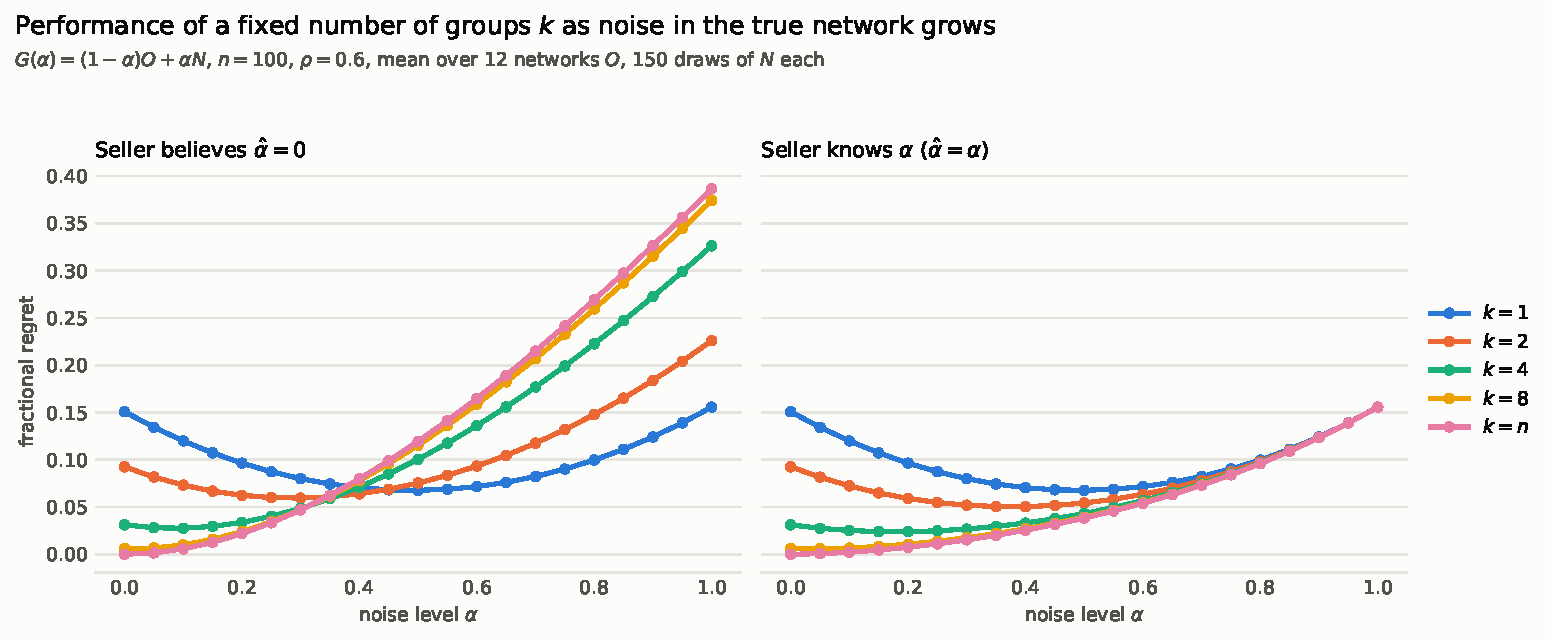
\includegraphics{Figures/Pricing_04/k_lines_vary_alpha.pdf}
\end{figure}   

\begin{figure}
    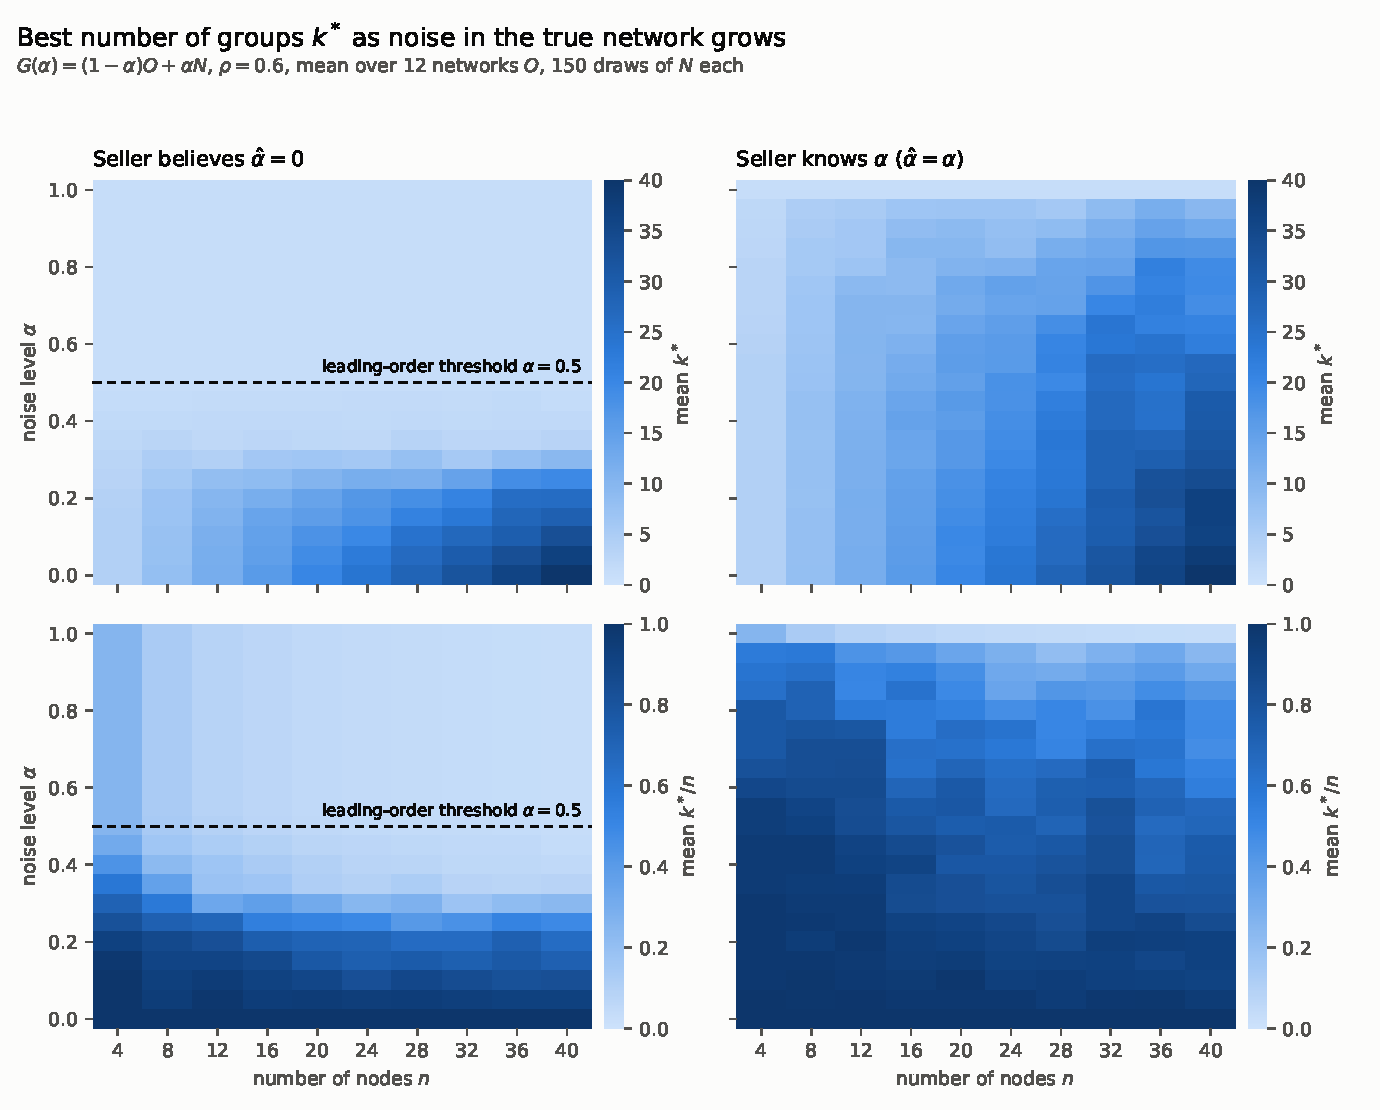
\includegraphics{Figures/Pricing_04/kstar_heatmap.pdf}
\end{figure}   








\begin{proposition}
    When $\alpha=1$, the optimal partition matrix is $R = \one^T$ and the optimal price is $\frac{a+c}{2}\one $.
\end{proposition}

From Theorem~\ref{thm:noisy-regret}, we pull out the second term and define $L(\alpha, \pricealpha ) \defeq (\delta \tb{p}(\alpha,R))^T W(\alpha,R) (\delta \tb{p}(\alpha, R))$. This term measures the expected regret due to uncertainty in the network. The next result gives an indication of how this regret changes as a function of the choice of partitioning. 

\begin{proposition}
    Let $R' \leatom R$. Then there exists $\rho > 0$ such that $L(\alpha, \pricealpha) \geq  L(\alpha, \pricealphaprime)$ for all $\alpha$.
\end{proposition}
The proof of this proposition, which may be found in the appendix, expands the regret into the contributions of walks of each length, shows that the result holds for the lowest-order terms, and bounds the remaining higher-order terms in terms of the lower-order terms. This result validates the intuition that choosing a finer pricing structure comes at the cost of higher regret due to noise. 

Next, we perform a numerical study to highlight these results. We consider a directed binary tree of height 4 as the base known network and take the noise to be entry-wise i.i.d.  To isolate the impact of uncertainty, we normalize the noise to have the same density as the original network. We simulate 1,000 different samples of noise across uncertainties ranging from zero to one. For each sample, we report the average fractional regret using different levels of coarseness. We include one-, two-, three-, and four-level pricing. For this experiment, we set $\rho=0.9, a=6, c=4$.
Figure~\ref{fig:klevel_numbies} showcases the results. The first panel shows the fractional regret, and we see that when noise is low, it is better to use more information. But as the noise increases, the prices that use fewer blocks are more volatile. When noise is zero, using 4 levels is best. But soon after, it is better to shift to three levels, two levels, and then one level.  We also observe that the fractional regret does not need to be monotonically increasing, as seen in the behavior of two-level pricing. The second panel abstracts away details and shows only how the best pricing level changes on average. This makes it clear that the duration a pricing level is best is not static. Notice also that this curve is continuous. It is continuous because it looks at the average best rank for that noise, but at each individual sample, there is a discrete best pricing level. 

\begin{figure}[H]
    \centering
    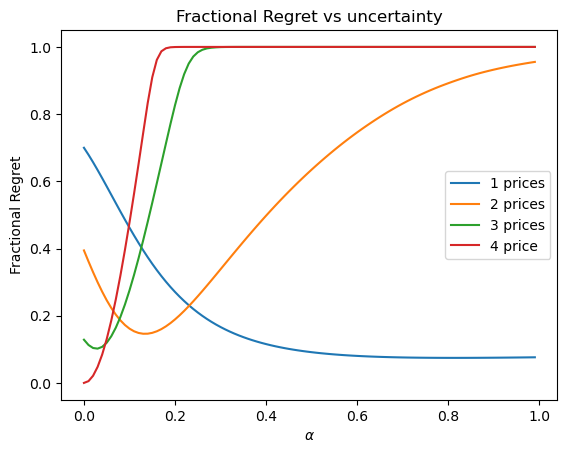
\includegraphics[width=0.45\textwidth]{Figures/Pricing/klevel/out2.png}
    \hfill 
    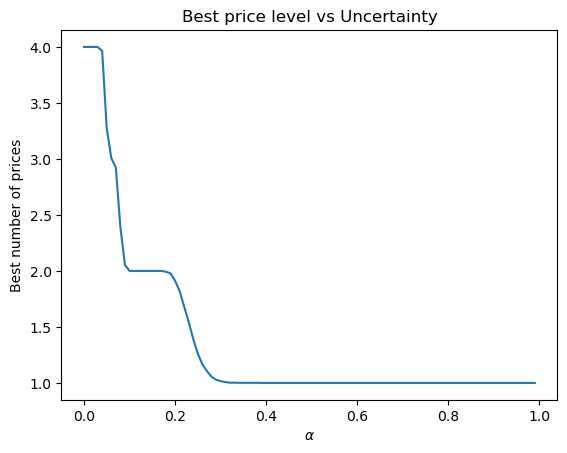
\includegraphics[width=0.45\textwidth]{Figures/Pricing/klevel/out1.png}
    % \subfloat[Fractional Regret of different pricing levels vs uncertainty]{ 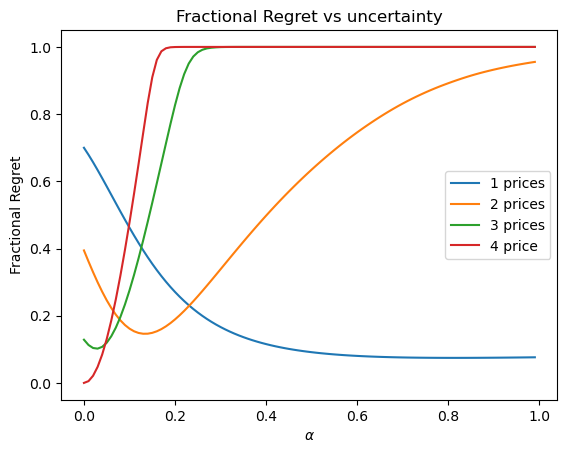
\includegraphics[width=0.45\textwidth]{Figures/Pricing/klevel/out2.png}
    %  }
    %  \hfill 
    %  \subfloat[Average Optimal  Pricing level vs uncertainty ]{
    %  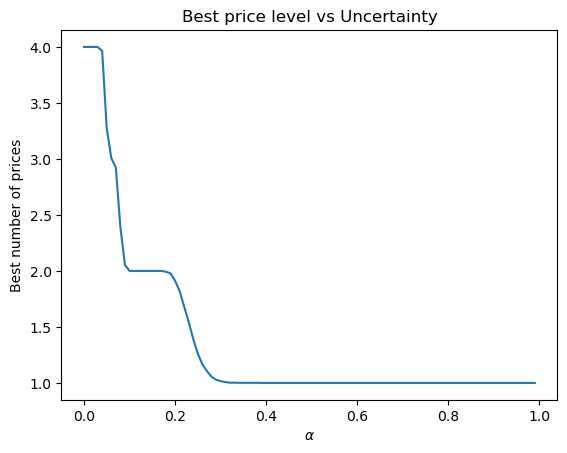
\includegraphics[width=0.45\textwidth]{Figures/Pricing/klevel/out1.png}
    %  }
    % \caption{a) Fractional Regret vs. noise of various pricing levels. Lower is better. b) How the best pricing level changes with noise.}
\end{figure}\label{fig:klevel_numbies}




\section{How to find Good partitions}

One practical problem for the merchant is to find the best partition.   This is, in general, a computationally hard combinatorial task.  

~\cite{candogan2012optimal} studied a variation where the merchant had to compute the optimal partition for two-level prices with a fixed high and low price. Instead of direct computation, the merchant must turn to approximation algorithms to find a strong partition.  

The usual way of partitioning the network into $k$ blocks would be to find $k$ communities. The problem is often stated as the modularity maximization problem~\cite{karrer2011stochastic,ball2011efficient}. While this problem is also NP-hard, several approximation algorithms have been used successfully, such as the Louvain algorithm~\cite{blondel2008fast}. However, such partitions perform poorly for price differentiation. We provide examples in the appendix\TODO{}. Community detection algorithms provide partitions that have tight internal connections based on the spatial arrangement of the network. Nodes that are nearby can get grouped together even if they differ drastically in their level of influence. This is why they perform poorly.

An interval heuristic for finding suitable partitions in practice is grouping consumers together by function, not location. The simplest way to do this is to group consumers based on their unconstrained price, which is itself a metric for how net influential a consumer is or is not. The proposed algorithm is a form of clustering over a one-dimensional space. Explicitly, we propose the following heuristic problem: 

\begin{definition}
    Given an integer $k$ and a vector $\tb{p}^*$ the clustering problem is to find a partitioning $R^*$ of  $[n]$ such that 
\end{definition}

While this problem may be solved with traditional k-means clustering algorithms~\cite{}, we can solve for the optimal solution to~\cite{} in polynomial time~\cite{}. In~\cite{}, we describe the full algorithm. A high-level view of the algorithm is shown in Figure~\ref{fig:03-pipeline}.

One desirable property of the prices found by clustering is that the partitions are formed into `intervals', in the sense that the blocks can be labeled and sorted such that every price in the first block is smaller than every price in the second, which is smaller than every price in the third, and so on. We call such a pricing structure an interval partition.
\begin{definition}
    A partition is said to be an \textbf{interval partition} with respect to $\tb{p}$ if, for all $i,j,\ell \in [n]$ with $p_i > p_j > p_\ell$, whenever $i$ and $\ell$ are in the same block, $j$ is as well.
\end{definition}
In practice, this solution performs very well over random matrices. However, we can construct counter-examples where the solution to this algorithm is not optimal. Furthermore, in this counter-example, the optimal partition is not even an interval partition. However, in~\cite{} we examine the impact of the highest-order terms of the Taylor expansion of profit and find that for low-order terms an analogous condition does hold. This suggests that the interplay of nodes in longer walks is what interferes with the interval property.


\begin{figure}
    \centering
    \resizebox{\textwidth}{!}{
        \begin{tikzpicture}[
  node distance = 2.0cm,
  %--- main pipeline boxes ---
  box/.style = {
    draw = black!65, line width = 0.8pt,
    fill = blue!8,
    rounded corners = 5pt,
    minimum width  = 3.0cm,
    minimum height = 1.5cm,
    align = center,
    font = \small
  },
  %--- algorithm sub-step ---
  subbox/.style = {
    draw = orange!70!black, line width = 0.7pt, dashed,
    fill = orange!7,
    rounded corners = 4pt,
    minimum width  = 2.8cm,
    minimum height = 1.1cm,
    align = center,
    font = \footnotesize
  },
  arr/.style  = {-{Stealth[length=7pt]}, line width=0.9pt},
  darr/.style = {-{Stealth[length=6pt]}, line width=0.7pt, dashed, orange!70!black}
]

%% ---- MAIN PIPELINE ----

\node[box] (pstar) {
  \textbf{Solve unconstrained}\\[3pt]
  $p^* = {(B+B^T)}^{-1}(aB + cB^\top)\mathbf{1}$
};

\node[box, right=2.0cm of pstar] (sort) {
  \textbf{Sort nodes by} $p^*$\\[3pt]
  $p^*_{\sigma(1)} \le \cdots \le p^*_{\sigma(n)}$
};

\node[box, right=2.0cm of sort] (partition) {
  \textbf{Optimal interval}\\
  \textbf{partition of order} $k$
};

\node[box, right=2.0cm of partition] (output) {
  \textbf{Prices}\\[3pt]
  one per interval\\
  $\hat{p}_{G_1},\dots,\hat{p}_{G_k}$
};

%% ---- ARROWS ----

\draw[arr] (pstar)     -- (sort);
\draw[arr] (sort)      -- (partition);
\draw[arr] (partition) -- (output);

%% ---- ALGORITHM SUB-STEP ----

\node[subbox, below = 1.1cm of partition] (alg) {
  \textbf{Algorithm}\\[2pt]
  $O(kn^2)$ DP\\
  over cut-points\\
  $\sigma(i_1), \sigma(i_2), \dots$
};

\draw[darr] (alg) -- (partition);

%% ---- INTERVAL ILLUSTRATION (below the number line) ----

% \begin{scope}[yshift = -4.0cm]

%   % axis
%   \draw[->, line width=0.6pt, gray!60] (-0.3,0) -- (10.5,0);
%   \node[gray!60, font=\footnotesize] at (10.7,0) {$p^*$};

%   % example sorted values (7 nodes)
%   \foreach \x/\lbl in {
%       0.6/$p^*_{\sigma(1)}$,
%       1.5/$p^*_{\sigma(2)}$,
%       2.6/$p^*_{\sigma(3)}$,
%       4.1/$p^*_{\sigma(4)}$,
%       5.3/$p^*_{\sigma(5)}$,
%       7.2/$p^*_{\sigma(6)}$,
%       8.9/$p^*_{\sigma(7)}$
%   }{
%     \fill[blue!50!black] (\x, 0) circle (2.2pt);
%     \node[font=\tiny, below=4pt] at (\x, 0) {\lbl};
%   }

%   % cut points (k=3 intervals)
%   \foreach \cx in {3.35, 6.25}{
%     \draw[red!70!black, line width=0.9pt, dashed] (\cx,-0.35) -- (\cx,0.35);
%   }

%   % interval braces / shading
%   \foreach \xa/\xb/\clr/\lbl in {
%       0.3/3.2/blue!15/{$G_1$},
%       3.5/6.1/green!15/{$G_2$},
%       6.4/9.1/orange!18/{$G_3$}
%   }{
%     \fill[\clr, rounded corners=2pt, opacity=0.5]
%       (\xa,-0.18) rectangle (\xb, 0.18);
%     \node[font=\footnotesize\bfseries] at ({(\xa+\xb)/2}, 0.42) {\lbl};
%   }

%   % caption
%   \node[align=center, font=\footnotesize\itshape, gray!70!black]
%     at (5.1,-0.85)
%     {Nodes sorted by $p^*$; vertical dashed lines are the optimal cut-points ($k = 3$)};

% \end{scope}

\end{tikzpicture}


% \definecolor{Col1}{HTML}{4E79A7}   % blue   – group 1
% \definecolor{Col2}{HTML}{F28E2B}   % orange – group 2
% \definecolor{Col3}{HTML}{E15759}   % red    – group 3

% \begin{tikzpicture}[
%   pbox/.style={
%     draw=gray!60, rounded corners=3pt,
%     minimum width=3.0cm, minimum height=1.1cm,
%     fill=blue!8, font=\small, align=center},
%   dpbox/.style={
%     draw=gray!55, rounded corners=3pt,
%     minimum width=3.5cm, minimum height=1.3cm,
%     fill=orange!7, font=\small, align=center},
%   harr/.style={-{Stealth[length=5pt]}, semithick, gray!70},
%   varr/.style={-{Stealth[length=4pt]}, thin, gray!45, dashed},
%   bpanel/.style={draw=gray!25, fill=gray!5, rounded corners=3pt, line width=0.5pt},
% ]

% %% ═══════════════════════════════════════════════════════════════════════════
% %% Layer 1 – pipeline boxes  (y = 0)
% %% ═══════════════════════════════════════════════════════════════════════════
% \node[pbox] (A) at (0,   0) {Compute\\$p^*$};
% \node[pbox] (B) at (4.5, 0) {Sort $p^*$\\(ascending)};
% \node[pbox] (C) at (9.0, 0) {Partition into\\$k$ intervals};

% \draw[harr] (A) -- (B)
%   node[midway, above, font=\scriptsize, text=gray]{rank nodes};
% \draw[harr] (B) -- (C)
%   node[midway, above, font=\scriptsize, text=gray]{$\arg\max_{\mathcal{R}}$};

% %% ═══════════════════════════════════════════════════════════════════════════
% %% Layer 2 – DP callout  (y ≈ −2.0)
% %%   centred between B and C (x = 6.75), width 3.5 cm → x ∈ [5.0, 8.5]
% %%   height 1.3 cm → y ∈ [−1.35, −2.65]
% %%   B arrow (x=4.5) passes 0.5 cm left of box;  C arrow (x=9.0) 0.5 cm right
% %% ═══════════════════════════════════════════════════════════════════════════
% \node[dpbox] (DP) at (6.75, -2.00) {
%   Optimal $k$-interval partition by DP: $O(n^2 k)$\\[3pt]
%   {\scriptsize$V(i,j)=\max_{l<i}\!\bigl[V(l,j{-}1)+\pi_{l+1:i}\bigr]$}
% };

% %% Thin note-line from B→C arrow (gap at x=6.75) down to DP box
% \draw[thin, gray!40, -{Stealth[length=3pt]}]
%   (6.75, -0.14) -- (DP.north);

% %% ═══════════════════════════════════════════════════════════════════════════
% %% Layer 3 – price-vector bar charts  (base y = −5.20, scale = 1.60)
% %%   6 nodes · bar 0.28 cm · stride 0.34 cm · span 1.98 cm · centred at cx
% %%
% %%   Example prices (∈ [0,1]):
% %%     node order :  0.70  0.20  1.00  0.40  0.15  0.60
% %%     sorted asc :  0.15  0.20  0.40  0.60  0.70  1.00
% %%     k=3 groups (2 nodes each)
% %% ═══════════════════════════════════════════════════════════════════════════

% %% ── Background panels ──────────────────────────────────────────────────────
% \foreach \cx in {0, 4.5, 9.0}{
%   \draw[bpanel] ({\cx-1.18}, -5.42) rectangle ({\cx+1.18}, -3.10);
% }

% %% ── A: unsorted p* ──────────────────────────────────────────────────────────
% \foreach \i/\h in {0/0.70, 1/0.20, 2/1.00, 3/0.40, 4/0.15, 5/0.60}{
%   \fill[gray!55, draw=gray!30, line width=0.4pt]
%     ({-0.99+\i*0.34}, -5.20)
%     rectangle ({-0.71+\i*0.34}, {-5.20+\h*1.60});
% }

% %% ── B: sorted ascending ─────────────────────────────────────────────────────
% \foreach \i/\h in {0/0.15, 1/0.20, 2/0.40, 3/0.60, 4/0.70, 5/1.00}{
%   \fill[gray!55, draw=gray!30, line width=0.4pt]
%     ({3.51+\i*0.34}, -5.20)
%     rectangle ({3.79+\i*0.34}, {-5.20+\h*1.60});
% }

% %% ── C: colored by interval ──────────────────────────────────────────────────
% \foreach \i/\h/\col in {
%     0/0.15/Col1,  1/0.20/Col1,
%     2/0.40/Col2,  3/0.60/Col2,
%     4/0.70/Col3,  5/1.00/Col3}{
%   \fill[\col!75, draw=\col!40, line width=0.4pt]
%     ({8.01+\i*0.34}, -5.20)
%     rectangle ({8.29+\i*0.34}, {-5.20+\h*1.60});
% }

% %% ── Interval bracket lines and labels (panel C) ─────────────────────────────
% %% G1: bars 0–1 → x ∈ [8.01, 8.63]
% %% G2: bars 2–3 → x ∈ [8.69, 9.31]
% %% G3: bars 4–5 → x ∈ [9.37, 9.99]
% \draw[Col1!90, line width=1.5pt] (8.01, -5.36) -- (8.63, -5.36);
% \draw[Col2!90, line width=1.5pt] (8.69, -5.36) -- (9.31, -5.36);
% \draw[Col3!90, line width=1.5pt] (9.37, -5.36) -- (9.99, -5.36);
% \node[font=\scriptsize, text=Col1!90] at (8.32, -5.57) {$\mathcal{G}_1$};
% \node[font=\scriptsize, text=Col2!90] at (9.00, -5.57) {$\mathcal{G}_2$};
% \node[font=\scriptsize, text=Col3!90] at (9.68, -5.57) {$\mathcal{G}_3$};

% %% ── Panel sub-labels (A, B) ─────────────────────────────────────────────────
% \node[font=\scriptsize\itshape, text=gray!70] at ( 0,  -5.57) {node order};
% \node[font=\scriptsize\itshape, text=gray!70] at (4.5, -5.57) {ascending $p^*$};

% %% ── Shared price axis ───────────────────────────────────────────────────────
% \draw[-{Stealth[length=3pt]}, gray!50, thin]
%   (-1.32, -5.20) -- (-1.32, -3.28)
%   node[above, font=\tiny, text=gray]{$p_i^*$};
% \draw[gray!35, thin] (-1.37, -5.20) -- (-1.27, -5.20);
% \node[left, font=\tiny, text=gray] at (-1.37, -5.20) {$c$};
% \draw[gray!35, thin] (-1.37, -3.60) -- (-1.27, -3.60);
% \node[left, font=\tiny, text=gray] at (-1.37, -3.60) {$a$};

% %% ═══════════════════════════════════════════════════════════════════════════
% %% Connecting arrows  (pipeline → bar chart panels)
% %% A and B pass left/right of the DP box;  C passes to its right
% %% ═══════════════════════════════════════════════════════════════════════════
% \draw[varr] (A.south) -- (0,   -3.12);
% \draw[varr] (B.south) -- (4.5, -3.12);
% \draw[varr] (C.south) -- (9.0, -3.12);

% \end{tikzpicture}

    }
\end{figure}\label{fig:03-pipeline} 



\definecolor{fn}{HTML}{2F5D8C}
\definecolor{cm}{HTML}{6B7280}

\SetKwProg{Fn}{Function}{}{}
\SetKwFunction{Main}{\textcolor{fn}{\textsc{ClusterPricing}}}
\SetKwFunction{KM}{\textcolor{fn}{\textsc{OneDimKMeans}}}
\SetKwInOut{Input}{Input}
\SetKwInOut{Output}{Output}
\SetKwComment{Comment}{\color{cm}$\triangleright$\ }{}
\SetKwComment{tcc}{\color{cm}$\triangleright$\ }{}
\SetCommentSty{textit}
\SetAlgoNlRelativeSize{-1}
\setlength{\algomargin}{1.6em}

\newcommand{\wss}{\operatorname{SS}}


\begin{algorithm}[H]
\caption{Group pricing by 1D clustering of the optimal prices}
\DontPrintSemicolon
\Input{Network $G\in\mathbb R_{\ge 0}^{n\times n}$, coupling $\gamma$, price bounds $a>c$, number of groups $k\le n$}
\Output{Groups $\mathcal G_1,\dots,\mathcal G_k$ and group prices $\bar p_1,\dots,\bar p_k$}
\BlankLine
\Fn{\Main{$G,\gamma,a,c,k$}}{
  \BlankLine
  \tcc{\textbf{Step 1.}\ Unconstrained optimal prices}
  $B \leftarrow (I-\gamma G)^{-1}$,\quad $M \leftarrow B+B^{\top}$\;
  $q \leftarrow aB\one + cB^{\top}\one$\;
  $p^{*} \leftarrow M^{-1}q$ \Comment*[r]{solve $Mp^*=q$}
  \BlankLine
  \tcc{\textbf{Step 2.}\ Sort the nodes by optimal price}
  $\sigma \leftarrow \textsc{Argsort}(p^{*})$ \Comment*[r]{$p^*_{\sigma_1}\le\dots\le p^*_{\sigma_n}$, any $O(n\log n)$ sort}
  $x_i \leftarrow p^{*}_{\sigma_i}$ for $i=1,\dots,n$\;
  \BlankLine
  \tcc{\textbf{Step 3.}\ Cluster the sorted prices into $k$ contiguous groups}
  $(b_0,b_1,\dots,b_k) \leftarrow$ \KM{$x,\,k$} \Comment*[r]{$0=b_0<b_1<\dots<b_k=n$}
  \BlankLine
  \tcc{\textbf{Step 4.}\ Form the groups and their optimal prices}
  $\mathcal G_j \leftarrow \{\sigma_{b_{j-1}+1},\dots,\sigma_{b_j}\}$ for $j=1,\dots,k$\;
  $R_{jv}\leftarrow \one[v\in\mathcal G_j]$ for $j=1,\dots,k$,\ $v=1,\dots,n$ \Comment*[r]{$R\in\{0,1\}^{k\times n}$}
  $\bar p \leftarrow (RMR^{\top})^{-1}Rq$ \Comment*[r]{$M$-projection of $p^*$ onto group-constant prices}
  \Return{$(\mathcal G_1,\dots,\mathcal G_k),\ \bar p$}\;
}
\end{algorithm}

\newpage
\begin{algorithm}[H]
\caption{Exact 1D $k$-means on sorted values: $O(n^2k)$ time, $O(nk)$ space}
\DontPrintSemicolon
\Input{Sorted values $x_1\le\dots\le x_n$, number of groups $k\le n$}
\Output{Cut points $0=b_0<b_1<\dots<b_k=n$ minimizing $\sum_{j=1}^{k}\wss(b_{j-1},b_j)$}
\BlankLine
\Fn{\KM{$x,k$}}{
  \BlankLine
  \tcc{Prefix sums, so any block cost takes $O(1)$}
  $P_0\leftarrow 0$,\ $P^{(2)}_0\leftarrow 0$\;
  \For{$i=1$ \KwTo $n$}{
    $P_i \leftarrow P_{i-1}+x_i$,\quad $P^{(2)}_i \leftarrow P^{(2)}_{i-1}+x_i^2$\;
  }
  $\wss(l,i) := \big(P^{(2)}_i-P^{(2)}_l\big)-\dfrac{(P_i-P_l)^2}{i-l}$ \Comment*[r]{within-block sum of squares of $x_{l+1},\dots,x_i$}
  \BlankLine
  \tcc{$V(i,j)$ = least cost of splitting $x_1,\dots,x_i$ into $j$ contiguous blocks}
  $V(0,0)\leftarrow 0$;\quad $V(i,0)\leftarrow+\infty$ for $i\ge1$\;
  \For{$j=1$ \KwTo $k$}{
    \For{$i=j$ \KwTo $n$}{
      $V(i,j)\leftarrow \displaystyle\min_{\,j-1\,\le\, l\,<\, i}\ \Big\{\,V(l,j-1)+\wss(l,i)\,\Big\}$\;
      $\mathrm{cut}(i,j)\leftarrow \displaystyle\arg\min_{\,j-1\,\le\, l\,<\, i}\ \Big\{\,V(l,j-1)+\wss(l,i)\,\Big\}$ \Comment*[r]{start of the last block}
    }
  }
  \BlankLine
  \tcc{Backtrack the cut points}
  $b_k\leftarrow n$\;
  \For{$j=k$ \KwTo $1$ \textbf{step} $-1$}{
    $b_{j-1}\leftarrow \mathrm{cut}(b_j,\,j)$\;
  }
  \Return{$(b_0,b_1,\dots,b_k)$}\;
}
\end{algorithm}

\medskip\small
\noindent\textbf{Remarks.}
Step~3 is exact for the 1D $k$-means cost: optimal 1D clusters are contiguous in sorted order, and the cost is additive across blocks.
It is a surrogate for the true regret $\mathrm{Reg}(R)=\tfrac12\min_{x}\|p^*-R^\top x\|_M^2$, which couples the groups through $M$.
With $\wss^*$ the optimal $k$-means value,
\[
\tfrac12\lambda_{\min}(M)\,\wss^*\;\le\;\mathrm{Reg}(\text{best $k$-partition of any shape})\;\le\;\mathrm{Reg}(\text{Algorithm 1})\;\le\;\tfrac12\lambda_{\max}(M)\,\wss^*,
\]
so Algorithm~1 is within a factor $\lambda_{\max}(M)/\lambda_{\min}(M)$ of optimal, and the left-hand side is a computable certificate.
The total cost is $O(n^3)$ for Step~1, $O(n\log n)$ for Step~2, $O(n^2k)$ for Step~3 and $O(n^2k+k^3)$ for Step~4.

Consider the following algorithm sketch. 

We can give a coarse bound for the performance of this algorithm. 
\begin{theorem}
    Let SS be the optimal within-group sum of squares and $R_{alg}$ be the resulting output of Algorithm~\cite{} then 
    \[ \frac{\mathrm{Reg}(\tb{p}(0,R_{alg}))}{ \mathrm{Reg}(\tb{p}(0,R^*))} \leq \kappa(B+B^T) \]

    Furthermore, there is an additive regret over the $R^*$ of
    \[ \Pi(0, \tb{p}(0,R^*)) - \Pi(0, \tb{p}(0,R_{alg})) \leq \frac{1}{8} (\lambda_{\max} - \lambda_{\min} ) \frac{n}{k^2} ( \max(\tb{p}^* ) - \min(\tb{p^*})) \] 
\end{theorem}
\textit{Proof idea.} This proof consists of constructing multiple inequalities where terms are primarily bounded either by the largest (smallest) eigenvalues of $B+B^T$ or as a result of the algorithm minimizing the spread of each block. The last result uses the fact that as the number of blocks increases, the spread of each block is non-increasing, thus improving the bound.


This theorem first shows that the algorithm produces a solution with a competitive ratio of at most the condition number of the matrix $B+B^T$. In practice, this is a loose upper bound. The second result shows that the regret versus the best $k$-level partition scales with three things: the gap between the largest and smallest eigenvalues, the size of the network, and the total spread between the high and low prices. However, it is scaled by a factor of $\frac{1}{k^2}$, so, holding other factors fixed, increasing $k$ quickly decreases the regret.


\subsubsection{Numerical Simulation}

\begin{figure}[H]
    \centering
    \caption{Fractional regret as a function of noise for $k$-level prices with various $k$. Lower is better. }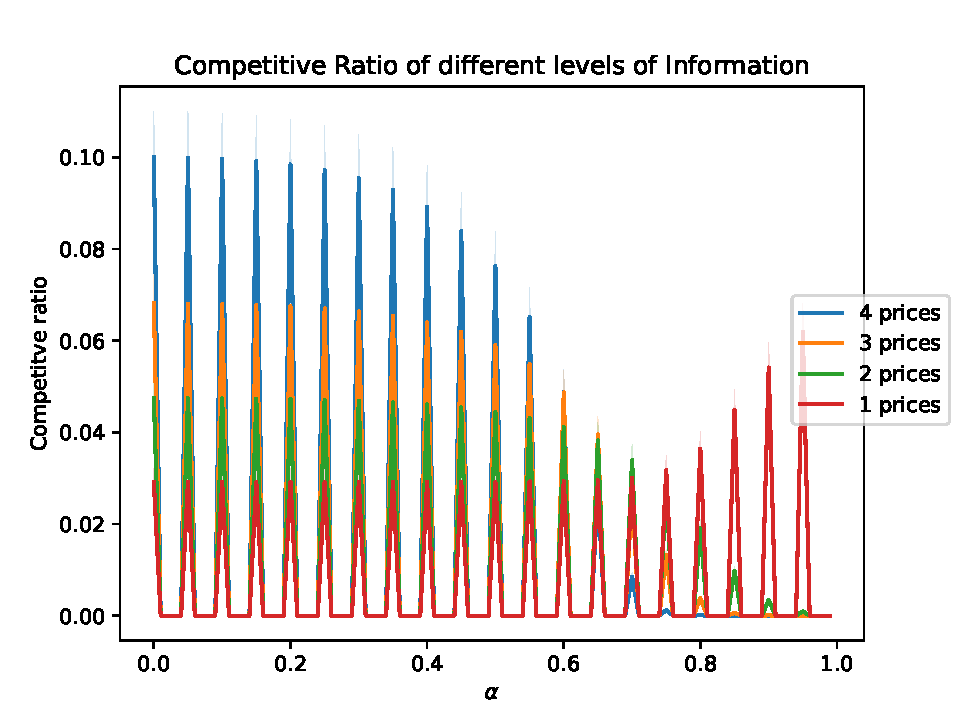
\includegraphics[width=0.45\linewidth]{Figures/Pricing/klevel/klevel.pdf}
\end{figure}\label{fig:k-prices}



We now showcase how $k$-level prices behave in practice. We consider networks of size 20. The observed part of the network will be a directed acyclic graph with random edge weights between nodes. The unobserved portion will be an Erd\H{o}s--R\'enyi network. We will plot the fractional regret compared to the clairvoyant price. Each run consists of varying $\alpha$, and therefore the weight between the two networks from $0$ to $1$. We perform $1,000$ runs and compute the fractional regret for using the uniform price, $2$ prices, $4$ prices, $5$ prices, and full non-clairvoyant pricing. The results are shown in Figure~\ref{fig:k-prices}. We find the partition $R$ to use for $2,4$, and $5$ prices by the modified K-Means++ algorithm. 


There are several phenomena showcased in this example. At low noise, higher fidelity prices are better but deteriorate as the noise increases. Around $\alpha\approx0.2$, the merchant should switch to five prices. With increasing $\alpha$ it should switch to three prices, then two, then one price.  We also note that the fractional regrets are non-monotonic in the noise. This means that the behavior of the fractional regret of the $k$-level prices found through the modified K-Means++ algorithm compared to the clairvoyant price at intermediate noise is complex.



To determine if this is a reasonable idea, we will compare it to modularity-based methods. The Louvain Community Detection Algorithm is a popular method of finding communities. This algorithm finds communities such that there is dense linkage inside a community and a sparsity of communication between different communities. 

We test over small networks such that the optimal partition can be reasonably found by brute force. For both the Louvain method and the degree clustering method, we ask how frequently the found partition lines up exactly with the profit-maximizing partition. In addition, we report how much fractional regret, on average, each algorithm yields. We do this for networks of size 8 with 300 different trials of random networks. In these trials, we run the Louvain method on the networks $G+G^T$ and $B+B^T$. We compare the performance for two-level pricing as well as four-level pricing. Parameters were set to $a=7,c=2, \rho=0.95$.


\begin{table}
    \centering
    \begin{tabular}{ccc}
        \toprule
        Name & Average Fractional Regret $\%$ & Accuracy \\
        \midrule
        Flow method &   $2.08$ &  $240/300$ \\
        Community ($G+G^T$) & $66.24$ & 3/300 \\
        Community ($B+B^T$) & $26.81$ &   67/300\\
        \bottomrule
    \end{tabular}
    \caption{Performance of different methods for finding a partition with two prices.}
    \begin{tabular}{ccc}
        \toprule
        Name & Average Fractional Regret $\%$ & Accuracy \\
        \midrule 
        Degree clustering method &   $5.3$ &  $160/300$ \\
        Community ($G+G^T$) & $42.1$ & 31/300 \\
        Community ($B+B^T$) & $42.82$ &   52/300 \\
        \bottomrule 
    \end{tabular}
    \caption{Performance of different methods for finding a partition with four prices.}
\end{table}\label{tab:placeholder}




We observe that the degree clustering method is significantly better at the task of finding profit-maximizing partitions. It achieves lower regret, finds the best solution $80\%$ of the time for the small network, and has, on average, low regret compared to the community-based detection methods. We do, however, observe that the performance of the flow-based method degrades as we increase the number of blocks, even though it still has lower regret than the alternatives. The reason for this gap is that the Louvain method places nearby nodes into the same community regardless of how starkly different they are in terms of net influence. However, the degree clustering method places consumers with similar influence together even if they are distant. Consumers with similar influence would be charged more similar prices in the unconstrained problem.

\subsection{Granularity of Partitions}
By Theorem~\ref{thm:noisy-regret} the merchant's expected profit depends upon the quality and granularity of the partition. In the absence of noise, we quantify the performance of partitions of different granularities. This performance is completely governed by the first term of the expected profit in Theorem~\ref{thm:noisy-regret}. We also compare the second term in the expected profit that captures the loss due to lack of knowledge about $\alpha$. Lower loss implies that a partition is more robust to noise. These two terms demonstrate the trade-offs between optimality and robustness. If the merchant overly relies on the network $G$, it overfits and loses profit when noise levels are high. If it is too cautious, it will miss out on potential profit when noise levels are low.

To compare partitions, we use the refinement order $R' < R$ and the covering relation $R' \leatom R$ from Section~\ref{sec:partitions}. Recall that the finest partition is $R = I$ and the coarsest is $R = \one^T$. The optimal price for the coarsest partition is the optimal uniform price, $\tb{p}_0 = \frac{a+c}{2} \one$.

Our first result compares the profits under partitions when there is no noise. We show that for all pairs of partitions, when we have full knowledge of the network, using the finer partition is better. When noise isn't an issue, using a finer $R$ allows for a strictly larger feasible region for prices, and the merchant is free to leverage this information more fully. Furthermore, when $R'$ covers $R$, we can state the precise amount of change in the profit.

For block labels $i, j \in [k]$, let $\delta(i,j) \in \mathbb{R}^k$ be defined by ${\delta(i,j)}_m = \begin{cases} 1 & \text{ if } m=i \\
-1 & \text{ if } m=j \\
0 & \text{ else. }
\end{cases}$
\begin{theorem}
    Let $R' < R$. Then
    \[ \Pi( 0, \pricezeroprime) \leq \Pi(0, \pricezero)\]

    In particular, if $R' \leatom R$, then 
    \[ \Pi(0, \pricezero) -  \Pi(0, \pricezeroprime) = \frac{(a-c)^2}{4} \frac{ (\pricezero - \pricezeroprime)^2 }{\delta(i,j)^T W(0,R)^{-1}  \delta(i,j)} \] 

\end{theorem}

The theorem implies that under no noise $R=I$ is the optimal partition. Next, we show the other extreme. When $\alpha = 1$, the merchant knows nothing about the network, and uniform pricing performs best. This is because there is no structure to exploit, and all consumers are equal in expectation.

We can also note that all $k$-level prices are projections of the optimal price onto subspaces defined by the partition and the network. Let $\proj{R}{B} \defeq R^T {\left( R (B+B^T)R^T \right)}^{-1} R (B+B^T)$. Below, we list some of the properties of this matrix.
\begin{proposition}
    $\proj{R}{B}$ is idempotent i.e. 
    \begin{enumerate}
        \item $(\proj{R}{B})^2 = \proj{R}{B}  $
    \end{enumerate}
\end{proposition}
These properties can be easily verified via direct algebra. Furthermore, we can state properties about how $\proj{R}{B}$ and $\proj{R'}{B}$ interact if $R' < R$.
\begin{proposition}
    Let $R' < R$ be two partitions. Then $\proj{R}{B} \proj{R'}{B} = \proj{R'}{B} \proj{R}{B} = \proj{R'}{B} $
\end{proposition}

That is to say, the projection matrices commute, and their product reduces to the projection onto the coarser space. Geometrically, the intuition is that if we have two subspaces $S_1 \subset S_2$, then projecting a vector onto $S_1$ gives the same result as projecting onto $S_2$ and then $S_1$, or onto $S_1$ and then $S_2$. This last projection is idempotent for any vector already in $S_1$. 

This projection matrix view helps us clarify how prices and profits relate between various partitions. 
\begin{lemma}
    The optimal partition price can be expressed as 
    \[\tb{p}(0,R) = \proj{R}{B} (B+B^T)^{-1} (aB+cB^T) \one = \proj{R}{B} \tb{p}^*\]
\end{lemma}

As a corollary, we have that: 
\begin{corollary}
    Let $R' < R$. Then \[\tb{p}(0,R') = \proj{R'}{B} \proj{R}{B} \tb{p}^* = \proj{R'}{B} \tb{p}(0,R)\]
\end{corollary}

The regrets can then be written as follows: 
\begin{corollary}
    Let $R' < R$. Then the regret of using $R'$ instead of $R$ is $\langle d, d\rangle_{B+B^T}$ where $d = \tb{p}(0,R) - \tb{p}(0,R') = \left( \proj{R}{B} - \proj{R'}{B} \right) \tb{p}^*$.
\end{corollary}


\section{Low-Order Results}



\subsection{Low-order results}

In this section, we study the series expansion of the pricing and profit structure in terms of length of walks. These approximations provide insights into the structure of the problem. \TODO{MORE}

We begin by expressing the series expansion of the price and profit. 

\begin{theorem}
    Given a partition, $R$, as $\rho \to 0$ the price is approximated by 
    \begin{align*}
        \tb{p}(0,R) &= \frac{a+c}{2} \one \\ 
        &+ \gamma R^T (RR^T)^{-1} R (G-G^T) \one \\ 
        &+ \gamma^2 \left( 2 (G^2 - (G^T)^2) - (G+G^T) R (RR^T)^{-1} R (G+G^T) \right)\one \\
        &+ O(\rho^3 )
    \end{align*}
\end{theorem}



\begin{theorem}
    Given a partition $R$, as $\rho \to 0$ the profit is approximated by
    \begin{align*}
        \Pi(0, \pricezero) &= \frac{(a-c)^2}{8} n & \text{Order 0 }\\
        &+ \gamma \frac{(a-c)^2}{8} \one^T G \one & \text{Order 1}\\
        &+ \gamma^2 \frac{(a-c)^2}{8} \one^T \left( G^2 + \frac{1}{4} (G-G^T)^T R^T(RR^T)^{-1} R (G-G^T) \right) \one & \text{Order 2} \\
        &+ O(\rho^3) \\
    \end{align*}

        where, as before, $\gamma = \frac{2\rho}{\|G+G^T\|}$.

\end{theorem}

One implication of this result is that the interval property holds up through second order. This means that for all networks, if the impact of longer walks decays quickly ($\rho \to 0$), then the best partition is one that places nodes into interval partitions based on the vector $(G-G^T)\one$. 

\begin{theorem}
    As $\rho\to 0 $, the optimal partition into $k$ parts is an interval partition with respect to $(G-G^T)\one$.
\end{theorem}
\textit{Proof idea.} The core of this proof is based on the low-order profit expression. We take the only term that depends upon the partition and show that if the optimal partition were not an interval partition, then there would be an improving swap of two nodes, and thus the partition would not be optimal.



